\documentclass{article}
\usepackage{url}
\usepackage{amsmath,bm}%
\usepackage{amsfonts}%
\pagestyle{empty}
\setlength{\textwidth}{7in}
\setlength{\oddsidemargin}{-.5in}
\setlength{\evensidemargin}{-.5in}
\setlength{\topmargin}{-.75in}
\setlength{\textheight}{9.4in}

\newcommand{\beaa}{\begin{eqnarray*}}
\newcommand{\eeaa}{\end{eqnarray*}}
\newcommand{\bea}{\begin{eqnarray}}
\newcommand{\eea}{\end{eqnarray}}
\def\E{\mathop{\rm E\,}\nolimits}
\def\Var{\mathop{\rm Var\,}\nolimits}
\def\Cov{\mathop{\rm Cov\,}\nolimits}
\def\Corr{\mathop{\rm Corr\,}\nolimits}
\def\logit{\mathop{\rm logit\,}\nolimits}
\newcommand{\eid}{{\stackrel{\cal{D}}{=}}}
\newcommand{\cip}{{\stackrel{{P}}{\to}}}
\def\bR{\mathbb{R}}     % real line

%%%%%%%%%%
% From http://www.disc-conference.org/disc1998/mirror/llncs.sty
\def\vec#1{\mathchoice{\mbox{\boldmath$\displaystyle\bf#1$}}
{\mbox{\boldmath$\textstyle\bf#1$}}
{\mbox{\boldmath$\scriptstyle\bf#1$}}
{\mbox{\boldmath$\scriptscriptstyle\bf#1$}}}
%%%%%%%%%%


\usepackage{Sweave}
\begin{document}

\begin{center}
{\bf STAT 515}

{\bf Example of MCMC with full conditional calculations}

\end{center}

This example comes from {\it Markov Chain Monte Carlo in Practice}
by Gilks, Richardson, and Spiegelhalter (1996, first edition), pages 75--76.

Suppose 
\begin{eqnarray*}
Y_1, \ldots, Y_n &\stackrel{\rm iid}{\sim} & N(\mu, \tau^{-1}) \\
\mu & \sim & N(0,1) \\
\tau & \sim & \mbox{Gamma}(2,1),
\end{eqnarray*}
and $\mu$ and $\tau$ are independent (that is, the prior density for
$(\mu, \tau)$ is the product of the individual densities).
Let us find the full conditional distributions for $\mu$ and $\tau$.  First, a bit of 
preliminary setup:

The likelihood function is the joint density of the data (given the parameters),
viewed as a function of the parameters:
\[
L(\mu, \tau) = \prod_{i=1}^n f(Y_i \mid \mu, \tau) =
\prod_{i=1}^n \frac{\sqrt{\tau}}{\sqrt{2\pi}} \exp\{ -\tau(Y_i-\mu)^2/2 \} =
	(2\pi)^{-n/2} \tau^{n/2} \exp \left\{ -\tau \sum_{i=1}^n (Y_i - \mu)^2 /2 \right\}.
\]
To find the joint density of $(\vec Y, \mu, \tau)$, we multiply $f(\vec Y \mid \mu, \tau)$ 
(the likelihood) by the prior:
\[
p(\vec Y, \mu, \tau) = (\mbox{constant}) \times 
\tau^{n/2} 
\exp \left\{ -\tau \sum_{i=1}^n (Y_i - \mu)^2 /2 \right\} 
\exp\{ -\mu^2/2 \} \tau \exp^{-\tau}.
\]

If the data $\vec Y$ are observed, then in a Bayesian framework our attention focuses on
the conditional density of $(\mu, \tau)$ given $\vec Y$.  This may be written
\[
p(\mu, \tau \mid \vec Y) =  
\frac{p(\vec Y, \mu, \tau)}{p(\vec Y)} =
\frac{p(\vec Y, \mu, \tau)}{\int\int p(\vec Y, \mu^*, \tau^*)\, d\mu^* d\tau^*},
\]
but the denominator above isn't really important for our purposes 
(because it does not involve $\mu$ or $\tau$), so we may simply write
\[
p(\mu, \tau \mid \vec Y) \propto p(\vec Y, \mu, \tau).
\]

Now we can finally talk about the full conditionals.  For $\mu$, we obtain
\[
p(\mu \mid \tau, \vec Y) = 
\frac{p(\mu, \tau \mid \vec Y)}{p(\tau \mid \vec Y)},
\]
but once again the denominator does not involve $\mu$ so we can combine the expressions above
to write, as a function of $\mu$,
\[
p(\mu \mid \tau, \vec Y) \propto p(\vec Y, \mu, \tau) \propto
\exp \left\{ -\tau \sum_{i=1}^n (Y_i - \mu)^2 /2 \right\}  \exp\{ -\mu^2/2 \}.
\]
(We have ignored all of the factors in $p(\vec Y, \mu, \tau)$ that do not involve $\mu$.)
Similarly, as a function of $\tau$, the full conditional for $\tau$ satisfies
\[
p(\tau \mid \mu, \vec Y) \propto p(\vec Y, \mu, \tau)=
\tau^{n/2} 
\exp \left\{ -\tau \sum_{i=1}^n (Y_i - \mu)^2 /2 \right\} 
\tau \exp^{-\tau}.
\]

If we do a little bit of algebra, we get
\[
p(\mu \mid \tau, \vec Y) =
\exp \left\{ -\frac{ 1+ n\tau}{2} \left( \mu - \frac{\tau\sum_{i=1}^n Y_i}{1+n\tau} \right)^2 \right\}
\times (\mbox{stuff not involving $\mu$})
\]
as the full conditional density for $\mu$.  We recognize this!  It is a normal density function for 
$\mu$, where the mean is $\tau\sum_{i=1}^n Y_i/(1+n\tau)$ and the variance is
$1/(1+n\tau)$.  Or, in symbols,
\[
\mu \mid \tau, \vec Y \sim N \left( \frac{\tau\sum_{i=1}^n Y_i }{1+n\tau} ,
\frac{1}{1+n\tau} \right).
\]

Similarly, for $\tau$, we can do some algebra to obtain
\[
p(\tau \mid \mu, \vec Y) =
\tau^{1+(n/2)} 
\exp \left\{ -\tau \left( 1 + \frac12 \sum_{i=1}^n (Y_i - \mu)^2 \right) \right\} 
\exp^{-1/\tau}
\times (\mbox{stuff not involving $\tau$})
\]
as the full conditional, and we recognize this as a gamma density for $\tau$.  In symbols,
\[
\tau\mid \mu, \vec Y \sim \mbox{Gamma} \left( 
2+\frac n2,
1+\frac12\sum_{i=1}^n(Y_i - \mu)^2
\right).
\]

Let's use these facts to run a Markov chain.  
The goal will be to set up the chain using variable-at-a-time Metropolis-Hastings
in such a way that its stationary distribution is the posterior density $p(\mu, \tau \mid \vec Y)$.
The data $\vec Y$ are at 
\url{http://sites.stat.psu.edu/~dhunter/515/hw/MCMCexampleData.txt}
\begin{Schunk}
\begin{Sinput}
> y <- scan("http://sites.stat.psu.edu/~dhunter/515/hw/MCMCexampleData.txt")
\end{Sinput}
\end{Schunk}
First, we must initialize the chain using some $\mu^{(1)}$ and $\tau^{(1)}$.  Ideally, 
we could sample from the true stationary (posterior) distribution to do this, but if we
could do that, we wouldn't need MCMC!  So let's simply use $(\mu^{(1)}, \tau^{(1)}) =
(1,2)$, which are the prior means.  (We could also look at the data and take the starting values
to be the sample mean and the reciprocal of the sample variance. )
\begin{Schunk}
\begin{Sinput}
> iteration <- 1
> mu <- 1
> tau <- 2
> sumOfY <- sum(y) # We'll need this value repeatedly.
> n <- length(y)
\end{Sinput}
\end{Schunk}
We will now run 1000 steps of a Markov chain in which we sample $\mu^{(i+1})$ from
the full conditional based on $\tau^{(i)}$ and $\vec Y$, then sample $\tau^{(i+1)}$ from
the full conditional based on $\mu^{(i+1)}$ and $\vec Y$:
\begin{Schunk}
\begin{Sinput}
> while (iteration <= 1e3) {
+   tmp <- tau[iteration]
+   mu <- c(mu, rnorm(1, mean=sumOfY * tmp / (1+n*tmp), sd = sqrt(1 / (1 + n*tmp))))
+   tau <- c(tau, rgamma(1, shape=2+n/2, rate=1+sum((y-mu[iteration+1])^2)/2))
+   iteration <- iteration+1
+ }
\end{Sinput}
\end{Schunk}

Let us now check on some of the properties of our MCMC sample.  To get a sense of the 
shape of the sample, a simple scatterplot will help:
\begin{Schunk}
\begin{Sinput}
> plot(cbind(mu, tau))
\end{Sinput}
\end{Schunk}
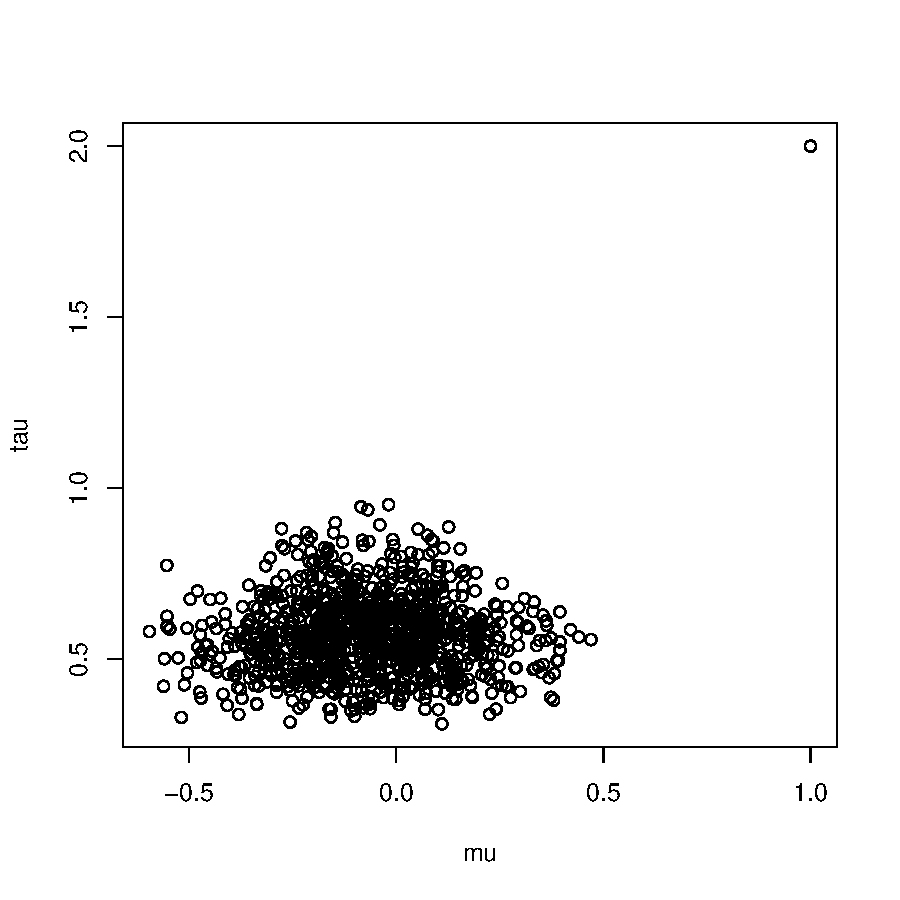
\includegraphics{MCMCexample-004}

The first thing we see is that the initial point is a long way from the rest of the points.  It 
is partly for this reason that sometimes a burnin period is used.  In our case, omitting the first
several points appears to be sufficient.  

Let us now look at some diagnostics to assess whether the Markov chain seems to be 
mixing well.  Simple plots of iteration against $\mu$ or iteration against $\tau$ (omitting the
first 5 points) give a pretty
good sense of this:
\begin{Schunk}
\begin{Sinput}
> par(mfrow=c(2,1))
> plot(mu[-(1:5)], type="l")
> plot(tau[-(1:5)], type="l")
\end{Sinput}
\end{Schunk}
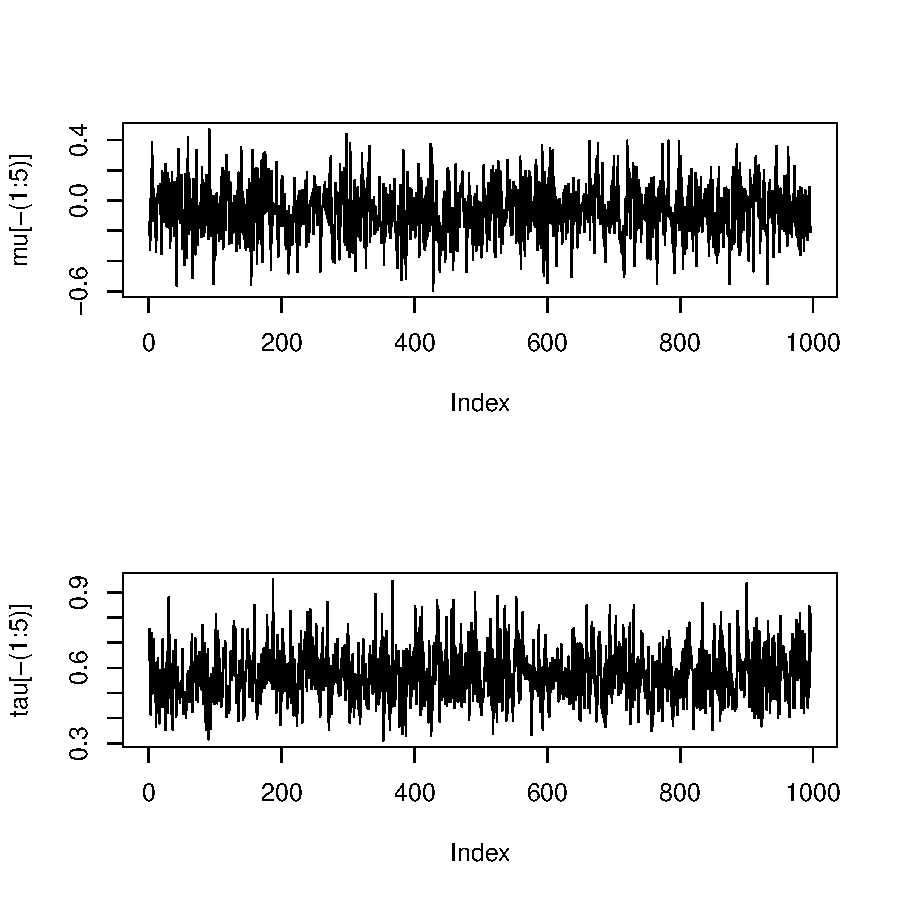
\includegraphics{MCMCexample-005}

These so-called traceplots do not give the sense of any overall trend, which might
indicate that the chain has not yet had a chance to adequately explore the posterior
parameter space.  (NB:  The plot gives no guarantees!  Some types of bizarre behavior
might not show up on a plot.)

Another helpful plot is a plot of the values of auto-correlation for various values of the 
``lag'' variable.  For lag $k$, the ACF (auto-covariance function) is the sample correlation
between the two samples $\theta_1, \ldots, \theta_{n-k}$ and $\theta_{1+k}, \ldots, \theta_n$.
In this case, the auto-correlation is close to zero even for a lag of one, which means that 
successive draws from this chain are nearly uncorrelated.  This is a very good thing! 
\begin{Schunk}
\begin{Sinput}
> par(mfrow=c(1,2))
> acf(mu)
> acf(tau)
\end{Sinput}
\end{Schunk}
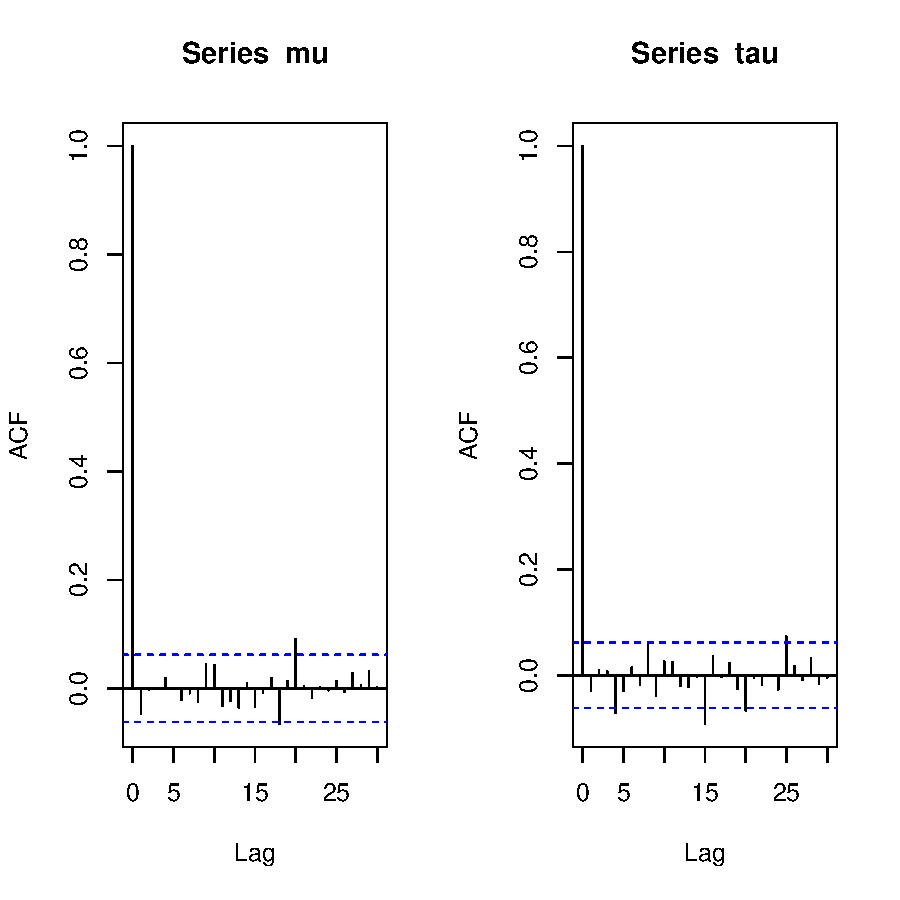
\includegraphics{MCMCexample-006}

Let us now focus on the $\mu$ parameter specifically.  The Bayes estimator of $\mu$ is equal to 
the mean of the posterior distribution; let us denote this value by $\tilde\mu$.  We do not actually
know what $\tilde\mu$ is, but we can estimate $\tilde\mu$ using our MCMC sample from the posterior.
Think of the following analogy:  If you have a random sample of size 1000 from a population with
mean $\tilde\mu$, then you would use the sample mean as the estimator of $\tilde\mu$, and by 
the central limit theorem you could also construct a 95\% confidence interval for $\tilde\mu$
using the sample mean plus or minus $1.96\hat s$, where $\hat s$ is an estimator of the
standard deviation of the sample mean (which is a random variable!).  In a similar way, we can use 
the sample mean of our $\mu$ sample---let's denote it by $\hat\mu$---to 
estimate $\tilde\mu$.  However, it is not always 
straightforward to estimate the standard deviation of  $\hat\mu$ because the MCMC sample is
not an i.i.d.~sample.  In fact, if we assume (simplistically) 
that the chain is stationary with distribution $\pi$, then
\[
\Var \hat\mu = \frac1 {n^2} \Var \sum_{i=1}^n \theta_i = 
\frac1n \Var_\pi \theta_i + \frac1{n^2} \sum_{k=1}^{n-1} (n-k) \Cov_\pi (\theta_1, \theta_{1+k}).
\]
This means that we would need more than an estimate of $\Var_\pi\theta_i$ in order to
estimate $\Var \hat\mu$.  Furthermore, if the covariances tend to be larger than zero, 
which is common in a Markov chain, ignoring them could lead to a dramatic underestimation
of the true variance---which in turn would lead to confidence intervals for $\tilde\mu$ that are 
too narrow!

In any event, as $m\to\infty$, any reasonable confidence interval for $\tilde\mu$ should get smaller.  
Such an interval captures only the error inherent in the MCMC approximation of the posterior (which diminishes as $m$ grows);
it does not capture the sampling distribution of the posterior distribution itself.  We have been assuming throughout this argument that
the data $\vec Y$ are fixed, but of course if we think more broadly, then $\vec Y$ is random, and a different sample leads to a different posterior.
Can we capture this source of variation, which is distinct from MCMC error?  One method is to create a 95\% credible interval, which is merely
a summary of the range of the middle 95\% of the posterior distribution.  For this purpose, we could proceed as follows:
\begin{Schunk}
\begin{Sinput}
> hist(mu, freq=FALSE, main="95% credible interval for mu")
> lines(density(mu), col=2)
> abline(v=print(quantile(mu, c(.025, .975))), lty=2, lwd=3)
\end{Sinput}
\begin{Soutput}
      2.5%      97.5% 
-0.4560731  0.3311048 
\end{Soutput}
\end{Schunk}
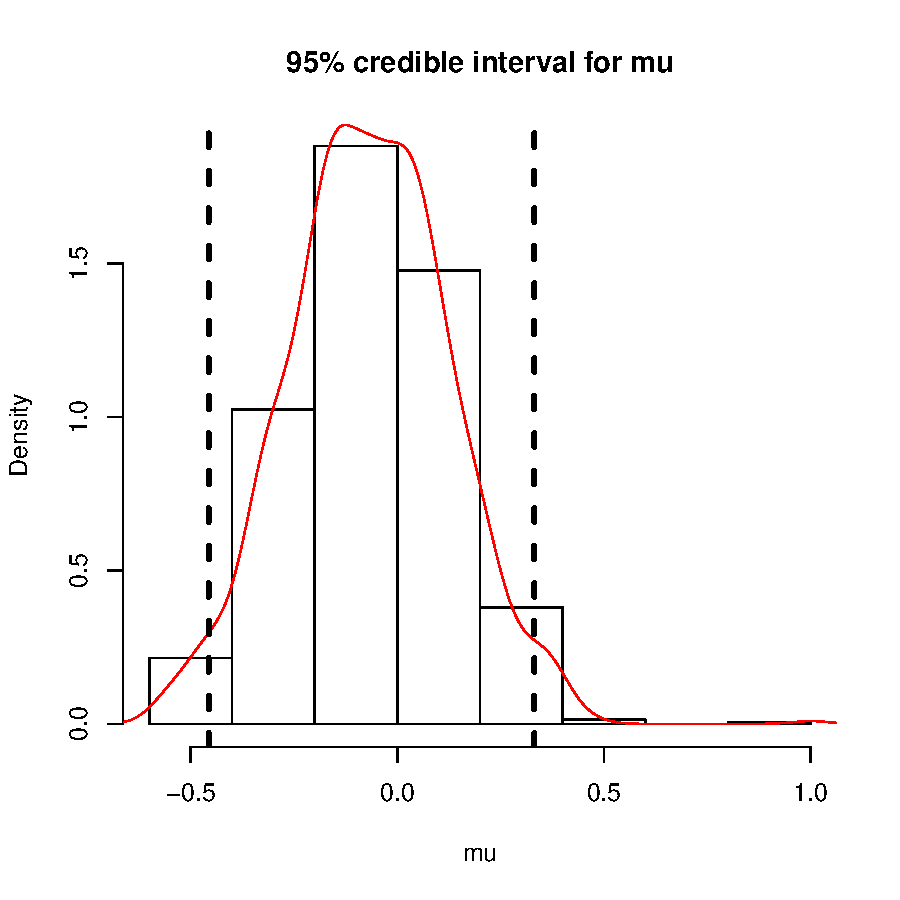
\includegraphics{MCMCexample-007}


\end{document}

